\documentclass[aspectratio=169,11pt]{beamer}
\usetheme{Madrid}
\usecolortheme{seahorse}
\usepackage{amsmath,amssymb}
\usepackage{tikz}
\usetikzlibrary{arrows.meta,positioning}
\usepackage{booktabs}

\setbeamertemplate{navigation symbols}{}
\setbeamerfont{footnote}{size=\tiny}

\title{WM-PLN: The World-Model Calculus}
\subtitle{A Mathematical Refoundation of PLN}
\author{Zar Goertzel\inst{1}\thanks{%
  Oru\v{z}i: AI collaboration using
  Claude Opus~4.6, GPT-5.4~Pro, Codex~5.4}}
\institute{Hyperon AGI Community Meeting}
\date{Addis Ababa, March 2026}

\newcommand{\hplus}{\oplus}
\newcommand{\mc}[1]{\textcolor{teal}{\textbf{Maple Court:} #1}}

\begin{document}

%% ══════════════════════════════════════════════════════
%% SLIDE 1: Title
%% ══════════════════════════════════════════════════════
\begin{frame}
\titlepage
\end{frame}

%% ══════════════════════════════════════════════════════
%% SLIDE 2: The Problem
%% ══════════════════════════════════════════════════════
\begin{frame}{The Problem: Truth Values Lose Structure}

PLN conflates three layers:
\begin{enumerate}
\item A \alert{probabilistic state} (the complete semantic object)
\item An \alert{evidence algebra} (the carrier)
\item \alert{Truth-value views} (strength, confidence --- lossy projections)
\end{enumerate}

\bigskip
When collapsed into $(s, c)$:
\begin{itemize}
\item Can't retract a faulty sensor's contribution
\item Can't explain \emph{why} the system believes what it believes
\item Can't tell ``strongly supported on little evidence'' from\\
      ``weakly supported on much evidence''
\end{itemize}

\end{frame}

%% ══════════════════════════════════════════════════════
%% SLIDE 3: The Hook
%% ══════════════════════════════════════════════════════
\begin{frame}{The Hook: More Data $\neq$ More Support}

\begin{center}
\Large
$e_1 = (1, 0)$ \qquad vs.\ \qquad $e_2 = (1, 1)$
\end{center}

\bigskip
\begin{itemize}
\item $e_2$ is \alert{more informed} (strictly more data)
\item $e_2$ is \alert{less supportive} (negative channel increased)
\item Strength \emph{decreases} even as evidence \emph{increases}
\end{itemize}

\bigskip
\begin{center}
\textbf{A system that stores only strength cannot see this.}
\end{center}

\end{frame}

%% ══════════════════════════════════════════════════════
%% SLIDE 4: The Move
%% ══════════════════════════════════════════════════════
\begin{frame}{The Move: Carry Evidence State}

Replace truth values with \alert{carried evidence state}.

\bigskip
\texttt{class WorldModel (State Query V : Type*) where}\\
\quad \texttt{revise \;: State -> State -> State}\\
\quad \texttt{empty \;\;: State}\\
\quad \texttt{extract : State -> Query -> V}

\bigskip
Four verbs: \alert{revise}, \alert{query}, \alert{forget}, \alert{explain}.

\bigskip
\mc{Each apartment carries a private evidence state.
Shared spaces carry a building-level state.}

\end{frame}

%% ══════════════════════════════════════════════════════
%% SLIDE 5: The Additive Regime
%% ══════════════════════════════════════════════════════
\begin{frame}{The Additive Regime}

The decisive law:
\[
  \mathrm{extract}(W_1 + W_2,\; q) =
  \mathrm{extract}(W_1, q) + \mathrm{extract}(W_2, q)
\]

\bigskip
\begin{theorem}[Profile-Hom Equivalence]
Additive world models $\cong$ additive monoid homomorphisms\\
$\mathrm{State} \to^+ (\mathrm{Query} \to V)$.
\end{theorem}

\bigskip
Every additive WM is an answer-profile generator.\\
This does \emph{not} trivialize the subject --- the hard work is\\
in proving when compiled shortcuts are exact.

\end{frame}

%% ══════════════════════════════════════════════════════
%% SLIDE 6: Three Carriers
%% ══════════════════════════════════════════════════════
\begin{frame}{Three Evidence Carriers}

\begin{center}
\begin{tabular}{lll}
\toprule
\textbf{Carrier} & \textbf{State} & \textbf{Domain} \\
\midrule
Binary & $(n^+, n^-)$ & Leak alarm counts \\
Dirichlet & $(\alpha_1, \ldots, \alpha_k)$ & Elevator health \\
Normal-Gamma & $(n, \sum x_i, \sum x_i^2)$ & Hallway temperature \\
\bottomrule
\end{tabular}
\end{center}

\bigskip
Same algebra, different carriers.\\
Revision $=$ addition of sufficient statistics.\\
Sleep consolidation: batch $=$ sequential (proved).

\end{frame}

%% ══════════════════════════════════════════════════════
%% SLIDE 7: The Pipeline
%% ══════════════════════════════════════════════════════
\begin{frame}{The End-to-End Pipeline}

\begin{center}
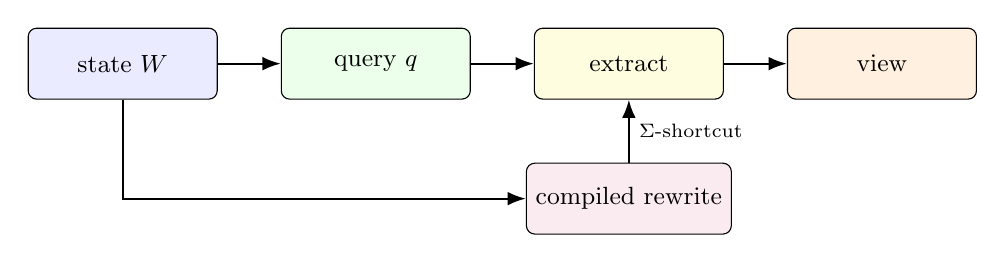
\begin{tikzpicture}[
  >=Latex, every node/.style={font=\small},
  box/.style={draw, rounded corners=3pt, minimum width=24mm,
              minimum height=9mm, align=center}
]
  \node[box, fill=blue!8] (state) {state $W$};
  \node[box, fill=green!8, right=8mm of state] (query) {query $q$};
  \node[box, fill=yellow!12, right=8mm of query] (extract) {extract};
  \node[box, fill=orange!12, right=8mm of extract] (view) {view};
  \node[box, fill=purple!8, below=8mm of extract] (rewrite) {compiled rewrite};

  \draw[->, thick] (state) -- (query);
  \draw[->, thick] (query) -- (extract);
  \draw[->, thick] (extract) -- (view);
  \draw[->, thick] (state) |- (rewrite);
  \draw[->, thick] (rewrite) -- node[right, font=\scriptsize]
    {$\Sigma$-shortcut} (extract);
\end{tikzpicture}
\end{center}

\bigskip
State is primary. Views are projections.\\
Compiled rewrites are certified shortcuts under side conditions.\\
Boundaries tell us where shortcuts \emph{cannot} be complete.

\end{frame}

%% ══════════════════════════════════════════════════════
%% SLIDE 8: The No-Go
%% ══════════════════════════════════════════════════════
\begin{frame}{The No-Go Theorem}

\begin{theorem}
Complete link evidence cannot, in general, be recovered
from local per-link surrogates alone.
\end{theorem}

\bigskip
This is a \alert{design theorem}, not an embarrassment.

\bigskip
It says:
\begin{itemize}
\item Local chaining is a shortcut, not the semantics
\item Side conditions ($\Sigma$) are not optional decoration
\item The additive regime identifies where shortcuts ARE exact
\end{itemize}

\end{frame}

%% ══════════════════════════════════════════════════════
%% SLIDE 9: Non-Additive Perimeter
%% ══════════════════════════════════════════════════════
\begin{frame}{The Non-Additive Perimeter}

Four revision regimes (not just additive):

\begin{description}
\item[Additive] Independent sources compose by $+$
\item[Overlap] Shared information $\Rightarrow$ correction term
\item[Trust-gated] Source authority gates the merge
\item[Coalition] Quorum required (semitopology)
\end{description}

\bigskip
Key result: \alert{additivity is recovered} when overlap is\\
small or non-actionable. \quad ($\sim$90 theorems, 0 sorry)

\end{frame}

%% ══════════════════════════════════════════════════════
%% SLIDE 10: KS Hypercube
%% ══════════════════════════════════════════════════════
\begin{frame}{The KS Probability Hypercube}

Each regime $=$ a vertex in the Knuth-Skilling hypercube:

\begin{center}
\begin{tabular}{llll}
\toprule
\textbf{Regime} & \textbf{Logic} & \textbf{Repr.} & \textbf{Vertex} \\
\midrule
Additive & Boolean & point & classical Bayesian \\
Overlap & Boolean & bounds & imprecise probability \\
Evidence & Heyting & 2D & PLN evidence \\
Trust-gated & Heyting & point & Heyting-point \\
\bottomrule
\end{tabular}
\end{center}

\bigskip
The WM algebra is \alert{not an ad-hoc design}.\\
It is the \emph{unique} algebra satisfying the KS axioms at each vertex.

\end{frame}

%% ══════════════════════════════════════════════════════
%% SLIDE 11: Formal Verification
%% ══════════════════════════════════════════════════════
\begin{frame}{Formal Verification}

\begin{center}
\Large\textbf{704+ theorems} \quad in Lean 4
\end{center}

\begin{center}
\Large\textbf{0 sorry} \quad\quad \textbf{0 native\_decide}
\end{center}

\bigskip
\begin{itemize}
\item Axioms: \texttt{propext}, \texttt{Classical.choice},
      \texttt{Quot.sound} only
\item 6 application domains, all kernel-checked
\item Every claim in the book $\to$ a specific Lean file
\item Build the file, verify the claim. Minutes, not trust.
\end{itemize}

\end{frame}

%% ══════════════════════════════════════════════════════
%% SLIDE 12: KS Triangle
%% ══════════════════════════════════════════════════════
\begin{frame}{The KS-Evidence-Measure Triangle}

\begin{center}
KS axioms
$\xrightarrow{\;\Theta = \mathrm{total}\;}$
$(\mathbb{R}_{\ge 0}^\infty, +)$
$\xrightarrow{\;\bullet\,\mathrm{dirac}\;}$
\texttt{Measure}
\end{center}

\bigskip
\begin{itemize}
\item Evidence carriers satisfy KS axioms (ordered, associative, monotone)
\item Representation $\Theta =$ total evidence function
\item Measure bridge $=$ representation $\circ$ Dirac weighting
\item \alert{Additivity at every vertex}: $\hplus$ on evidence, $+$ on reals, $+$ on measures
\end{itemize}

\bigskip
$\sigma$-additivity boundary: finitely additive $\not\Rightarrow$ $\sigma$-additive.\\
Proved non-derivable (KS counterexample).

\end{frame}

%% ══════════════════════════════════════════════════════
%% SLIDE 13: ProbLog Bridge
%% ══════════════════════════════════════════════════════
\begin{frame}{ProbLog = WM-PLN = BDD-WMC}

\begin{center}
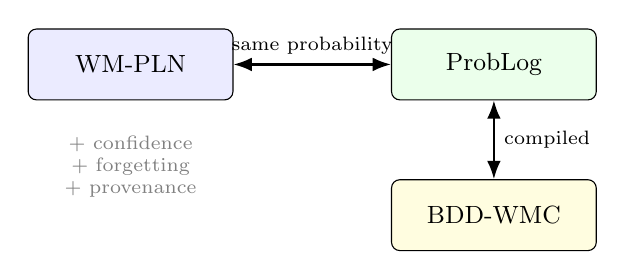
\begin{tikzpicture}[
  >=Latex, every node/.style={font=\small},
  box/.style={draw, rounded corners=3pt, minimum width=26mm,
              minimum height=9mm, align=center}
]
  \node[box, fill=blue!8] (wm) {WM-PLN};
  \node[box, fill=green!8, right=20mm of wm] (pl) {ProbLog};
  \node[box, fill=yellow!12, below=10mm of pl] (bdd) {BDD-WMC};

  \draw[<->, thick] (wm) -- node[above, font=\scriptsize]
    {same probability} (pl);
  \draw[<->, thick] (pl) -- node[right, font=\scriptsize]
    {compiled} (bdd);

  \node[font=\scriptsize, text=gray, align=center]
    at (0, -1.3) {$+$ confidence\\$+$ forgetting\\$+$ provenance};
\end{tikzpicture}
\end{center}

\bigskip
WM-PLN computes the \alert{same probabilities} as ProbLog\\
AND additionally supports revision, forgetting, sensitivity.\\
5,148 lines of BDD formalization. 0 sorry.

\end{frame}

%% ══════════════════════════════════════════════════════
%% SLIDE 14: Gas Sensor Drift
%% ══════════════════════════════════════════════════════
\begin{frame}{Application: Gas Sensor Drift Governance}

UCI Gas Sensor Array: 13,910 measurements, 36 months, 6 gases.

\bigskip
\begin{itemize}
\item WM-PLN is \alert{not replacing XGBoost}
\item It's a governance layer: when to retrain?
\item WM/XGBoost \alert{agreement gating}: AURC improves 0.385 $\to$ 0.374
\item Sequential replay: 64.5\% @ 23.9\% labels (cheap trigger)
\item Forgetting stale batches $\Rightarrow$ accuracy recovers
\end{itemize}

\end{frame}

%% ══════════════════════════════════════════════════════
%% SLIDE 15: UW-CSE
%% ══════════════════════════════════════════════════════
\begin{frame}{Application: UW-CSE Compatibility Gate}

Predict: \texttt{advisedBy(student, professor)}

\bigskip
\begin{tabular}{lrl}
\toprule
\textbf{Role} & \textbf{Evidence} & \textbf{Marginal} \\
\midrule
NeedAdvisor(s) & $\langle 3, 0 \rangle$ & 3 \\
CanAdvise(p) & $\langle 3, 0 \rangle$ & 3 \\
\alert{PairAffinity(s,p)} & $\langle 4, 0 \rangle$ & \alert{4} \\
MLN logit & $\langle 2, 2 \rangle$ & 2 \\
\midrule
\textbf{All roles} & $\langle 12, 2 \rangle$ & 6:1 \\
\textbf{Without PairAffinity} & $\langle 8, 2 \rangle$ & 4:1 \\
\bottomrule
\end{tabular}

\bigskip
PairAffinity is the \alert{gate}. Same \texttt{forget} pattern.

\end{frame}

%% ══════════════════════════════════════════════════════
%% SLIDE 16: Demand
%% ══════════════════════════════════════════════════════
\begin{frame}{Application: Demand-Directed Backward Chaining}

Chain: Collie $\to$ Dog $\to$ Mammal. Query: Mammal(Lassie).

\bigskip
\begin{center}
\begin{tabular}{lr}
\toprule
\textbf{Premise} & \textbf{Demand} \\
\midrule
\alert{Dog(Lassie)} (unknown) & \alert{1000} \\
B$\to$C rule & 210 \\
A$\to$B rule & 191 \\
Collie(Lassie) (known) & 50 \\
\bottomrule
\end{tabular}
\end{center}

\bigskip
After supply: demand \alert{contracts} 1000 $\to$ 240.\\
After forgetting Collie: demand \alert{reopens} 50 $\to$ 1000.

\end{frame}

%% ══════════════════════════════════════════════════════
%% SLIDE 17: PPLBench
%% ══════════════════════════════════════════════════════
\begin{frame}{PPLBench: Nine-Lane Validation}

\begin{itemize}
\item \textbf{Normal-Normal}: WM-PLN matches Stan exactly, $O(1)$ vs $O(N)$
\item \textbf{Dirichlet-Categorical}: exact conjugate, $< 10^{-15}$ error
\item \textbf{Noisy-OR}: semantic factor graph $\Rightarrow$ 3.0 PLL improvement
\item \textbf{Logistic/Robust}: Laplace approximation (honest boundary)
\end{itemize}

\bigskip
\begin{center}
\alert{Where conjugacy holds: exact and fast.}\\
\alert{Where it doesn't: the calculus says so.}
\end{center}

\end{frame}

%% ══════════════════════════════════════════════════════
%% SLIDE 18: What WM-PLN Gives
%% ══════════════════════════════════════════════════════
\begin{frame}{What the Refoundation Gives PLN}

\begin{enumerate}
\item \textbf{One kernel}: the posterior-state calculus
\item \textbf{Many views}: strength, confidence, intervals --- all projections
\item \textbf{Explicit $\Sigma$}: every compiled rule carries its assumptions
\item \textbf{Cleaner boundaries}: no-go theorems tell you where not to go
\item \textbf{Demand-directed control}: backward chaining by sensitivity
\item \textbf{Beyond subsumption}: compatibility-gated evidence decomposition
\end{enumerate}

\end{frame}

%% ══════════════════════════════════════════════════════
%% SLIDE 19: Big Picture
%% ══════════════════════════════════════════════════════
\begin{frame}{The Big Picture}

\begin{center}
\large
GSLT weight map $=$ WM extract
\end{center}

\bigskip
Every typed rewrite system (every GSLT) has a canonical\\
additive evidence algebra via multiset counting.

\bigskip
The WM calculus is not specific to probabilistic logic.\\
It is the \alert{evidence layer for any computational system}.

\bigskip
Replace $V$ with $\mathbb{C}$: quantum amplitudes.\\
Replace $V$ with intervals: imprecise probability.\\
The KS hypercube classifies which algebra you get.

\end{frame}

%% ══════════════════════════════════════════════════════
%% SLIDE 20: Thank You
%% ══════════════════════════════════════════════════════
\begin{frame}{Thank You}

\begin{center}
\large\textbf{WM-PLN: The World-Model Calculus}\\[6pt]
\normalsize
192-page book (community draft)\\
704+ theorems in Lean 4, 0 sorry\\
6 application domains\\[12pt]

\texttt{lean-projects/mettapedia/}\\[6pt]

\textit{``This overview shows the crystal.\\
The rest of the book turns the crystal in the light.''}
\end{center}

\end{frame}

\end{document}
